\documentclass[10pt]{amsart}

\usepackage[utf8]{inputenc}

\usepackage{algorithm}
\usepackage[noend]{algpseudocode}
\usepackage{amsfonts}
\usepackage{amsmath}
\usepackage{amssymb}
\usepackage{amsthm}
\usepackage[backend=biber, citestyle=numeric-comp, bibstyle=ieee]{biblatex}
\usepackage{changepage}
\usepackage{enumitem}
\usepackage{fancyhdr}
\usepackage[T1]{fontenc}
\usepackage{fullpage}
\usepackage[hidelinks]{hyperref}
\usepackage{mathtools}
\usepackage{physics}
\usepackage{thmtools}
\usepackage{tikz}
\usepackage{tikz-3dplot}
\usetikzlibrary{angles, cd, quantikz, quotes, patterns}
\usepackage{titlesec}
\usepackage{wasysym}

\usepackage{tikz-cd}

\usepackage{bookmark}
\usepackage[nameinlink]{cleveref}

\titleformat{\section}{\normalsize\bfseries}{\thesection}{1em}{}
\titleformat{\subsection}{\normalsize\bfseries}{\thesubsection}{1em}{}
\titleformat{\subsubsection}{\normalsize\bfseries}{\thesubsubsection}{1em}{}

\addbibresource{bibliography.bib}

\theoremstyle{definition}
\newtheorem{theorem}{Theorem}
\newtheorem{definition}{Definition}
\theoremstyle{remark}
\newtheorem{problem}[theorem]{Problem}
\newtheorem{lemma}[theorem]{Lemma}
\newtheorem{remark}[theorem]{Remark}
\newtheorem{observation}[theorem]{Observation}
\newtheorem{example}[theorem]{Example}
\newtheorem{corollary}[theorem]{Corollary}

\renewcommand{\qedsymbol}{\(\blacksquare\)}

\setlength{\parindent}{0pt}

\DeclareMathOperator{\controrot}{CR}
\DeclareMathOperator{\expectation}{E}
\DeclareMathOperator{\gf}{GF}
\DeclareMathOperator{\qft}{QFT}
\DeclareMathOperator{\rk}{rk}
\DeclareMathOperator{\defect}{def}
\DeclareMathOperator{\swapgate}{SWAP}
\DeclareMathOperator{\che}{CHE}
\DeclareMathOperator{\poly}{poly}
\DeclareMathOperator{\Span}{Span}
\DeclareMathOperator{\diag}{diag}

\newcommand{\djk}{\delta_{j, k}}
\newcommand{\tlk}{\tilde{\lambda_k}}

\newcommand{\evalat}[2]{\left.{#1}\middle|\right._{#2}}

% SOURCE: https://tex.stackexchange.com/questions/296151/double-head-and-hook-arrow
\newcommand{\hookdoubleheadrightarrow}{%
  \hookrightarrow\mathrel{\mspace{-15mu}}\rightarrow
}

\begin{document}
    \pagenumbering{gobble}

    valentinpi \hfill Last Change: \today{}

    \section*{A Short Dive into Adiabatic Quantum Computation and Adiabatic Grover}

    \textbf{Abstract.} \emph{Adiabatic Quantum Computation} (AQC) provides a different framework for Quantum Computing (QC) than \emph{Gate-based Quantum Computation} (GQC). In these notes, an overview of AQC and the Adiabatic equivalent of Grovers Algorithm is given.

    \textbf{Notation and Assumptions.} \(0 \in \mathbb{N}\). We work with a complex Hilbert space \(\mathcal{H}\) for our quantum mechanical model. \(L(\mathcal{H})\) denotes the bounded endomorphisms over \(\mathcal{H}\).

    \section{The Adiabatic Theorem}

    A quantum system is described by a state \(\ket{\psi}\in \mathcal{H}\) with \(\norm{\ket{\psi}} = 1\). Fixing the position and unfixing the time, the change of the system is described by the time-dependent Schrödinger equation
    
    \phantom{}

    \fbox{\parbox{\linewidth}{
    \begin{align}
        \frac{\partial}{\partial t} \ket{\psi(t)} = -\frac{i}{\hbar} H(t)\ket{\psi(t)}
    \end{align}
    }}
    
    \phantom{}

    with \(\hbar \in \mathbb{R}\) being the \emph{reduced Planck constant}, for some Hamiltonian path \(H\colon \mathbb{R}_{\geq 0} \to L(\mathcal{H})\), where we consider a Hamiltonian to be a positive-semidefinite Hermitian operator.
    \begin{definition}
        An eigenvalue \(\lambda \in \mathbb{R}\) of a Hamiltonian \(H \in L(\mathcal{H})\) is called an \emph{energy}. A state, associated with the lowest eigenvalue of \(H\), if it exists, is called a \emph{ground state}. The other states are called \emph{excited states}. Particles/Waves with multiple ground states are called \emph{non-degenerate}. When the time \(t\) is fixed, we also speak of \emph{instantaneous} eigenstates of a particle, due to the associated Hamiltonian being fixed in time.
    \end{definition}

    Let \(\varepsilon_0(t) \leq \varepsilon_1(t) \leq ...\) and \(\ket{\varepsilon_j(t)}\) for \(j \in \mathbb{N}\) denote eigenvalue-eigenstate pairs of the Hamiltonian of the associated particle/wave at a time point \(t\).\footnote{For a finite-dimensional space, one may ignore the remaining infinitely many energies.} The eigenvalue spectrum is used in quantum theory to encode energies of particles. Denote \(\Delta(t) \coloneqq \varepsilon_1(t) - \varepsilon_0(t) \geq 0\) as the instantaneous \emph{ground state gap}. We now now consider the particles behavior in a fixed time frame ending in a time \(t_f \in \mathbb{R}_{> 0}\).
    
    \phantom{}

    \fbox{\parbox{0.98\linewidth}{
        Suppose \(\ket{\psi(0)}\) is in the ground state of \(H(0)\). The \emph{adiabatic theorem} of QM roughly states, that, if the Hamiltonian path \(H\) changes ''slowly'', that then the resulting state \(\ket{\psi(t_f)}\) is also a ground state of \(H(t_f)\).
    }}
    
    \phantom{}

    We may remark, that this can be generalized for any excited state aswell. Such a slowly changing process can be implemented in practice. The idea of the theorem is somewhat natural, as the fact, that the Hamiltonian changes slowly, intuitively coincides with the preservation of the ground state property.
    
    However, the proof, or even the rigorous formulation, is rather hard\footnote{As described by Griffiths \cite{Griffiths}, but I cannot find the page right now. Not sure, if my physical version of the book is \emph{too new} or something.}. It is not clear, what ''slowly'' means here. The systems Hamiltonian is transformed via small perturbations, for instance. These perturbations can achieve any Hamiltonian path, Aharonov \cite[pp. 51-52]{Albash2016} even argued, that we can use them to add ''catalysts'', which can lower the total evolution time.

    \phantom{}
    \begin{minipage}{\linewidth}
        \centering
        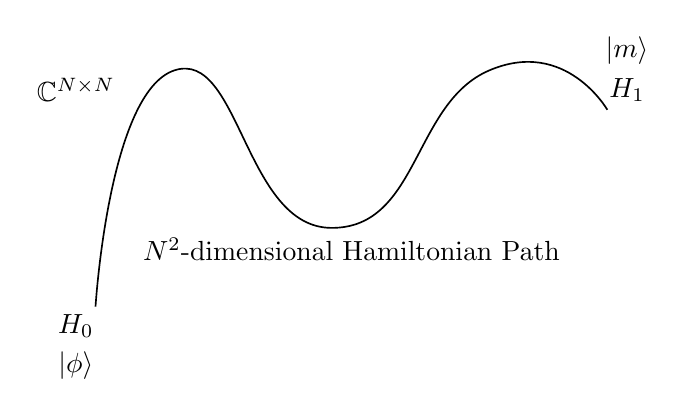
\begin{tikzpicture}[>=stealth, semithick]
            \node (0) at (0, 0) {\(H_0\)};
            \node (1) at (7, 3) {\(H_1\)};
            \node at ($(0)+(0, -0.5)$) {\(\ket{\phi}\)};
            \node at ($(1)+(0, 0.5)$) {\(\ket{m}\)};
            \draw plot [smooth, tension=1] coordinates { ($(0)+(0.25, 0.25)$) ($(0)+(1.25, 3.25)$) ($(0)+(3.25, 1.25)$) ($(0)+(5.25, 3.25)$) ($(1)+(-0.25, -0.25)$) };
            \node at (0, 3) {\(\mathbb{C}^{N \times N}\)};
            \node[below=0.25cm] at ($0.5*(0)+0.5*(1)$) {\(N^2\)-dimensional Hamiltonian Path};
        \end{tikzpicture}
    \end{minipage}

    \phantom{}
    
    The Hamiltonian path here that describes the energy changes of the particle over time is, for simplicity, the linear path given by
    \begin{align}
        H\colon [0, 1] \to L(\mathcal{H}), s \mapsto (1-s)H_0 + sH_1
    \end{align}

    \phantom{}

    \begin{minipage}{\linewidth}
        \centering
        \begin{tikzpicture}[>=stealth, semithick]
            \node (0) at (0, 0) {\(H_0\)};
            \node (1) at (7, 3) {\(H_1\)};
            \node at ($(0)+(0, -0.5)$) {\(\ket{\phi}\)};
            \node at ($(1)+(0, 0.5)$) {\(\ket{m}\)};
            \draw plot [smooth, tension=1] coordinates { ($(0)+(0.25, 0.25)$) ($(1)+(-0.25, -0.25)$) };
            \node[above left, rotate=23] at ($0.5*(0)+0.5*(1)$) {\(H\)};
            \node at (0, 3) {\(\mathbb{C}^{N \times N}\)};
        \end{tikzpicture}
    \end{minipage}

    \phantom{}

    with \(H_0, H_1 \in L(\mathcal{H})\) being the start and final Hamiltonians. The time here is restricted to \([0, 1]\) for normalization, but we can define a \emph{schedule} \(s\colon [0, t_f] \to [0, 1]\), s.t. \(H \circ s\colon [0, t_f] \to L(\mathcal{H})\) describes the actual physical change of the system. Optimizing the schedule to lower the evolution time \(t_f\) is desirable.

    \phantom{}
    
    There are several versions of the adiabatic theorem, we now consider one.

    \begin{theorem}
        Consider a quantum system \(\ket{\psi(\cdot)}\colon [0, 1] \to \mathcal{H}\) initialized in its ground state with a Hamiltonian path \(H\colon [0, 1] \to L(\mathcal{H})\) between \(H_0 \coloneqq H(0)\) and \(H_1 \coloneqq H(1)\).
        \begin{itemize}
            \item \(t_f \in \mathbb{R}_{> 0}\) (wlog. \(\neq 0\)) and \(s\colon [0, t_f] \to [0, 1]\) be a schedule.
            \item \(H(s)\) for all \(s \in [0, 1]\) always have a ground energy.
            \item \(\varepsilon_i(s)\) denote the \(i\)th eigenvalue of \(H(s)\) with \(\varepsilon_0(s) \leq \varepsilon_1(s) \leq ...\) for \(s \in [0, 1]\).
            \item \(\ket{\varepsilon_i(t)}\) denote the associated \(i\)th eigenvector of \(H(s)\).
            \item \(P(s)\) be the projector, that maps into the ground energy eigenroom of \(\varepsilon_0(t)\).
            \item \(P_{t_f}(s) = \ket{\psi(t)}\bra{\psi(t)}\) be the projector onto the simultaneous actual state.
            \item \(m(s)\) be the number of eigenvalues of \(P(s)\).
            \item \(H(s)\) be twice continuous-differentiable.
            \item \(H(s), \dot{H}(s), \ddot{H}(s)\) be bounded for any \(s \in [0, 1]\).
            \item \(\Delta(s) \coloneqq \varepsilon_1(s) - \varepsilon_0(s)\) be the ground state energy gap, where \(\min \Delta > 0\), i.e. the gap never vanishes.
        \end{itemize}
        Then, for any \(s \in [0, 1]\), we have
        \begin{align}
            \norm{P_{t_f}(s)-P(s)} \leq \frac{1}{t_f} \left(\evalat{\frac{m\norm{\dot{H}}}{\Delta^2}}{0} + \evalat{\frac{m\norm{\dot{H}}}{\Delta^2}}{s} + \int_0^s \left(\frac{m\norm{\ddot{H}}}{\Delta^2} + \frac{7m\sqrt{m}\norm{\dot{H}}^2}{\Delta^3}\right)\right)
        \end{align}
    \end{theorem}

    See the survey in \cite[p. 7]{Albash2016}. This version is not very precise, but rather simple to state in comparison to other versions. 
    The essential idea of AQC is thus to initialize a qubit state \(\ket{\psi} \in \mathbb{C}^N\), starting out with the Hamiltonian \(H_0\). This state is in some ground state of that Hamiltonian. The Hamiltonian is then slowly perturbed, according to the adiabatic theorem, to obtain a ground state of \(H_1\), which represents our solution Hamiltonian. As for the cost of the evolution, Aharonov et al. \cite[p. 3]{Albash2016} defined it to be
    \begin{align}
        t_f \max\norm{H}
    \end{align}

    As for optimality, there exists the following result: Defining the path length naturally as \(L \coloneqq \int_{t_0}^{t_1} \norm{\dot{H}(t)} \, dt\), it holds, that:
    \[
        t_f > \mathcal{O}(L/\min \Delta)
    \]

    \begin{table}[!hbtp]
        \begin{tabular}{c|c|c}
            Question & GQC & AQC\\
            \hline
            Which objects do we modify? & States & Hamiltonians\\
            How do we modify them? & Unitary matrices & Slow perturbations\\
            How do we determine the algorithm efficiency? & Number and locality of gates & \(t_f \max\norm{H}\)
        \end{tabular}

        \caption{Comparing GQC and AQC.}
    \end{table}

    \section{Adiabatic Grover}

    Let \(n \in \mathbb{N}_{\geq 1}\), \(N \coloneqq 2^n\). Consider a function \(f\colon \{0, 1\}^n \to \{0, 1\}\) with \(|f^{-1}(1)| = 1\). Let \(m \coloneqq f^{-1}(1)\). We want to obtain \(m\).

    The adiabatic version of Grovers Algorithm requires a Hamiltonian Path between
    \begin{align}
        H_0 \coloneqq E_N - \ket{\phi}\bra{\phi} \qquad H_1 \coloneqq E_N - \ket{m}\bra{m}
    \end{align}
    with \(\ket{\phi} \coloneqq H^{\otimes n}\ket{0}\). Both matrices are clearly Hermitian. It is important to note, that the final Hamiltonian \(H_1\) is our oracle, instead of \(f\). We can also denote \(H_1 = \diag(f(0), ..., f(m), ..., f(N-1))\).

    \phantom{}
    
    We first reason, why this evolution starts in a ground state. Observe, that initializing an \(n\)-qubit register to \(\ket{\phi}\) gives a ground state of \(H_0\). First, we have
    \begin{align}
        H_0\ket{\phi} = \ket{\phi} - \ket{\phi}\braket{\phi} = 0
    \end{align}
    The claim is due to \(H_0\) being positive-semidefinite, as we will now prove.
    \begin{definition}[Positive-Semidefinite and Positive-Definite Matrices]
        A Hermitian matrix \(A \in \mathbb{C}^{n \times n}\) is called \emph{positive-semidefinite}, if \(x^\dagger A x \geq 0\) for all \(x \in \mathbb{C}^n\). If the inequality is strict, then it is called \emph{positive-definite}.
    \end{definition}
    \begin{theorem}[Characterization of Positive-Semidefinite Matrices]
        The following statements are equivalent.
        \begin{enumerate}[label=(\roman*)]
            \item \(A\) is positive-semidefinite.
            \item \(\sigma(A) \subset \mathbb{R}_{\geq 0}\).
        \end{enumerate}
        where \(\sigma(A)\) denotes the spectrum of \(A\).
    \end{theorem}

    For the definition and the proof of the theorem see \cite[pp. 86-91]{Lyche}. The positive-semidefiniteness of \(H_0\) is not obvious. Let \(x \in \mathbb{C}^n\), \(\lambda \in \mathbb{R}\). The eigenvalue equation is
    \begin{align}
        H_0x = (E_N-\ket{\phi}\bra{\phi})x = \lambda x \leadsto \ket{\phi}\bra{\phi}x = (1-\lambda)x
    \end{align}
    This gives
    \begin{align}
        \frac{1}{N} \begin{pmatrix}
            \sum_{i=1}^N x_i\\
            ...\\
            \sum_{i=1}^N x_i
        \end{pmatrix} = (1-\lambda) \begin{pmatrix}
            x_1\\
            ...\\
            x_N
        \end{pmatrix}
    \end{align}
    in turn giving the condition
    \begin{align}
        \frac{1}{N} \sum_{i=1}^N x_i = (1-\lambda) x_1 = ... = (1-\lambda) x_N
    \end{align}
    If \(\sum_{i=1}^N x_i = 0\), then either \(\lambda = 1\) or \(x = 0\). That concerns the zero eigenvalues. For \(\lambda \neq 1\) and \(x \neq 0\), we have \(x_1 = ... = x_N\). If we assume wlog. \(x_1 \neq 0\), then we have
    \begin{align}
        1-\lambda = \frac{1}{N} \frac{\sum_{i=1}^N x_i}{x_i} = \frac{1}{N} \frac{Nx_1}{x_1} = 1
    \end{align}
    \(\lambda = 0\) thus yields the only other eigenvalue. We have \(\sigma(H_0) = \{0, 1\}\) with respective eigenroom dimensions \(1\) and \(N-1\) via the dimension formula \(N = \rk(H_0) + \defect(H_0)\), where \(\defect(H_0) \coloneqq \dim(\ker(H_0))\) is called the \emph{defect} of the linear map.

    As its eigenvalues thus are in \(\mathbb{R}_{\geq 0}\), we conclude, that \(0\) is the lowest eigenvalue, so \(\ket{\phi}\) is a ground state.

    \phantom{}

    As for \(H_1\), it holds, that \(\sigma(H_1) = \{0, 1\}\) with \(0\) being the energy of \(\ket{m}\) and the other eigenstates having energy \(1\). This can be read off directly, as \(H_1\) is a diagonal Hamiltonian. So when we start adiabatically evolving from the ground state \(\ket{\phi}\) of \(H_0\), we will reach the ground state \(\ket{m}\) of \(H_1\) via slow permutations in the time of the adiabatic theorem.

    \phantom{}
    
    We discuss two such paths.

    \subsection{Linear Interpolation}

    

    We define our path by
    \begin{align}
        H\colon [0, 1] \to \mathbb{C}^{N \times N}, t \mapsto (1-s)H_0+sH_1
    \end{align}

    Which is the simplest continuous Hamiltonian path. We start with the same initial state \(\ket{\phi}\).
    
    Denote \(\ket*{m^\perp} \coloneqq \sqrt{\frac{N}{N-1}}\left(\ket{\phi}-\frac{1}{\sqrt{N}}\ket{m}\right)\).

    ...

    \begin{align}
        t_f \gg \frac{3}{\Delta_{\text{min}}^2} = 3 \cdot N
    \end{align}

    So this schedule does not yield a speedup compared to the classical brute-force algorithm.

    \subsection{Exponential Ansatz}

    \printbibliography{}
\end{document}
